% Construction : E = (0, 0), F = (4, 0), D = (0, 3) — une unité vaut 2 cm.
% L'angle droit est en E ; l'hypoténuse est [DF], de longueur 10 cm. Le cosinus
% de l'angle en D est le quotient du côté adjacent [DE] par l'hypoténuse.
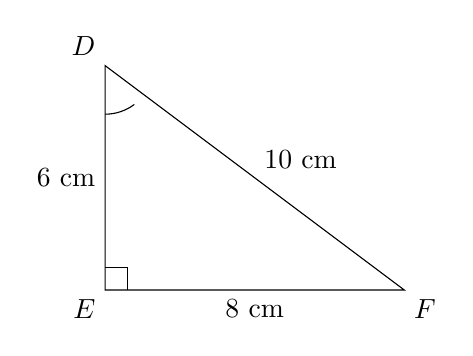
\begin{tikzpicture}[scale=0.95]
  \coordinate (E) at (0, 0);
  \coordinate (F) at (4, 0);
  \coordinate (D) at (0, 3);
  \draw (E) -- (F) -- (D) -- cycle;
  \draw (0.3, 0) -- (0.3, 0.3) -- (0, 0.3);
  \draw (0, 2.35) arc (-90:-53:0.65);
  \node[below left]  at (E) {$E$};
  \node[below right] at (F) {$F$};
  \node[above left]  at (D) {$D$};
  \node[left]  at (0, 1.5) {$6$ cm};
  \node[below] at (2, 0)   {$8$ cm};
  \node[above right] at (2, 1.5) {$10$ cm};
\end{tikzpicture}
